\section{Approach}
\label{sec:approach}
\begin{figure}[t]
\centering
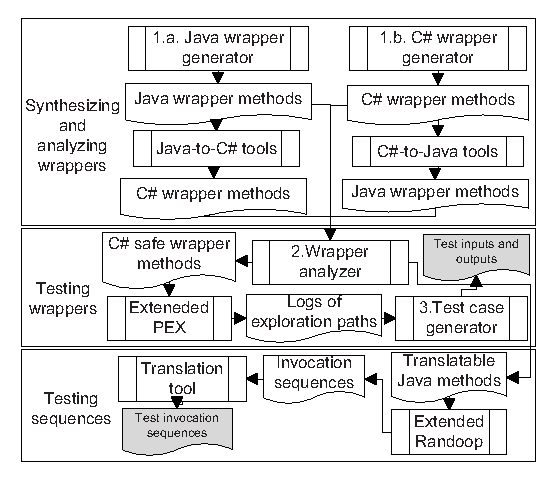
\includegraphics[scale=1,clip]{figure/approach.eps}\vspace*{-3ex}
 \caption{Overview of TeMAPI}\vspace*{-4ex}
 \label{fig:approach}
\end{figure}
Given a translation tool between Java and C\#, TeMAPI generates various test cases to reveal behavior differences of the tool's API mapping relations.
Figure~\ref{fig:approach} shows the overview of TeMAPI. It is able to test not only mapping relations of a single API invocation but also mapping relations of multiple API invocations.


%-------------------------------------------------------------------
\subsection{Translating Generated wrapper methods}
\label{sec:approach:generating}
Given a translation tool, TeMAPI first extracts its translatable API invocations. It is challenging to extract such invocations directly from translation tools for two factors: (1) different translation tools may follow different styles to describe API mapping relations. For example, as shown in Section~\ref{sec:introduction}, the API mapping relations of Java2CSharp are described in its mapping files, but the API mapping relations of sharpen are hard-coded in its source files. (2) commercial translation tools typically hide their API mapping relations in binary files. Due to the two factors, TeMAPI does not extract API mapping relations directly from translation tools, but chooses to analyze translated code of translation tools. In particular, TeMAPI generates a wrapper method for each API invocation and analyzes translated results for translatable API invocations. We do not use translation tools to translate existing projects for two considerations: (1) existing projects typically contain quite a small set of API invocations, so many API mapping relations may be not covered; (2) a single method of an existing project may invoke multiple API methods, so it may be difficult to analyze which methods are not mapped. TeMAPI relies on the reflection technique~\cite{maes1987concepts} provided by both Java and C\# to generate wrapper methods for translation.

\textbf{Static fields.} Given a public static field \CodeIn{f} of a class \CodeIn{C} whose type is \CodeIn{T}, TeMAPI generates a getter as follows:
\begin{CodeOut}%\vspace*{-2ex}
\begin{alltt}
 public T TestGet|f.name||no|()\{ return C.f; \}
\end{alltt}
\end{CodeOut}

If \CodeIn{f} is not a constant, TeMAPI generates a setter as follows:
\begin{CodeOut}%\vspace*{-2ex}
\begin{alltt}
 public void TestSet|f.name||no|(T v)\{ C.f = v; \}
\end{alltt}
\end{CodeOut}

\textbf{Non-static fields.} Given a public non-static field \CodeIn{f} of a class \CodeIn{C} whose type is \CodeIn{T}, TeMAPI generates a getter for each constructor \CodeIn{C(T1\ p1,\ldots, Tn\ pn)} of \CodeIn{C} as follows:
\begin{CodeOut}%\vspace*{-2ex}
\begin{alltt}
 public T TestGet|f.name||no|(T1\ c1,\ldots, Tn\ cn)\{
    C obj = new C(c1,\ldots, cn);
    return obj.f; \}
\end{alltt}
\end{CodeOut}

If \CodeIn{f} is not a constant, TeMAPI generates a setter as follows:
\begin{CodeOut}%\vspace*{-2ex}
\begin{alltt}
 public void TestSet|f.name||no|(T1\ c1,\ldots, Tn\ cn)\{
   C obj = new C(c1,\ldots, cn);
   obj.f = v; \}
\end{alltt}
\end{CodeOut}

In the preceding code, ``\CodeIn{|f.name|}'' denotes the name of \CodeIn{f}, and ``\CodeIn{|no|}'' denotes the corresponding number of generated wrapper method.

\textbf{Static methods.} Given a public static method \CodeIn{m(T1\ p1,\ldots,Tn\ pn)} of a class \CodeIn{C} whose return type is \CodeIn{Tm}, TeMAPI generates a wrapper method as follows:
\begin{CodeOut}%\vspace*{-2ex}
\begin{alltt}
 public Tm Test|m.name||no|(T1\ m1,\ldots, Tn\ mn)\{
   return C.m(m1,\ldots, mn); \}
\end{alltt}
\end{CodeOut}

\textbf{Non-static methods.} Given a public non-static method \CodeIn{m(T1\ p1,\ldots,Tn\ pn)} of a class \CodeIn{C} whose return type is \CodeIn{Tm}, TeMAPI generates a wrapper method for each constructor \CodeIn{C(Tv\ pv,\ldots, Tt\ pt)} of \CodeIn{C} as follows:
\begin{CodeOut}%\vspace*{-2ex}
\begin{alltt}
 public Tm Test|m.name||no|(T1\ m1,\ldots, Tn\ mn,
                            Tv cv, \ldots, Tt ct)\{
   C obj = new C(cv,\ldots, ct);
   return obj.m(m1,\ldots, mn); \}
\end{alltt}
\end{CodeOut}

In the preceding code, ``\CodeIn{|m.name|}'' denotes the name of \CodeIn{m(T1\ p1,\ldots,Tn\ pn)}.

TeMAPI put all generated wrapper methods for one API class $C$ into one generated class. For a Java-to-C\# tools, TeMAPI generates wrapper methods in Java as shown by the solid line in Figure~\ref{fig:approach}, and for a C\#-to-Java tools, TeMAPI generates wrapper methods in C\# as shown by the dotted line in Figure~\ref{fig:approach}. When generating methods, TeMAPI ignores generic API methods for simplicity. Besides, it ignores \CodeIn{unsafe} and \CodeIn{delegate} API methods and API methods whose parameters are marked as \CodeIn{out} or \CodeIn{ref} when generating C\# methods. Java does not have corresponding keywords, so there are typically not mapped. After TeMAPI generate wrapper methods, we translate them using a translation tool under experiments.

After generated code is translated, TeMAPI parses translated code and removes translated methods with compilation errors. For Java code, TeMAPI extends Eclipse's Java compiler to extract methods with compilation errors. For C\# code, TeMAPI extracts the list of compilation errors through the automation and extensibility interfaces of Visual Studio. Using remained methods, TeMAPI tests single API invocations (Section~\ref{sec:approach:single}). From remained methods, TeMAPI also analyzes the list of translatable API invocations for a given translation tool. Using the list, TeMAPI further tests API invocation sequences (Section~\ref{sec:approach:sequence}).


%for validate API mapping relations of the translation tool. To achieve this, TeMAPI first remove all translated methods with compilation errors. For translated methods in Java, TeMAPI implements a Eclipse plug-in that uses on Eclipse JDT compiler\footnote{\url{http://www.eclipse.org/jdt/}} for the list of compilation errors. For translated methods in C\#, TeMAPI implements a Visual Studio.Net add-in to retrieve the list of compilation errors from the error-list view of Visual Studio.Net. Both Eclipse JDT compiler and Visual Studio.Net cannot list all methods with compilation errors in a single build. After each iteration of removing methods, TeMAPI re-build these methods until it removes all methods with compilation errors.
%
%After methods with compilation errors are removed, TeMAPI compares generated code with translated code for the validate API mapping relations of a translation tool. Based on translated code and validate API mapping, TeMAPI removes generated methods whose corresponding translated methods have compilation errors. We refer to those removing wrapper methods as safe methods.


%-----------------------------------------------------------------
\subsection{Testing Single API Invocations}
\label{sec:approach:single}

Pex~\cite{tillmann2008pex} is a white-box test generation tool for .Net based on dynamic symbolic execution. Basically, Pex repeatedly executes a method under test, so that it explores all feasible paths of the method. To reduce the efforts to explore paths, Pex leverage various search strategies. For example, Xie \emph{et al.}~\cite{xie09:fitness} propose a search strategy called Fitnex that uses state-dependent fitness values to guide path exploration of Pex.

TeMAPI extends Pex, so that it generates test cases for detecting behavior differences of single invocations. In particular, for each translated C\# wrapper methods, TeMAPI records the inputs and the corresponding output when Pex searches each path. Based on recorded inputs and outputs, TeMAPI generates Java test cases to ensure each mapped API invocations produce the same output give the same inputs.
For example, TeMAPI records that given a integer whose value is 0, the output of the \CodeIn{TestvalueOf57sm} method in C\# is ``0''. Based on the preceding input and output, TeMAPI generates a Java test case for the \CodeIn{testvalueOf57sm} method in Java as follows:

\begin{CodeOut}%\vspace*{-2ex}
\begin{alltt}
public void testvalueOf57sm7()\{
  sketch.Test_java_lang_String obj =
      new sketch.Test_java_lang_String();
  int m0 = 0;
  Assert.assertEquals("0", obj.testvalueOf57sm7(m0));\}
\end{alltt}
\end{CodeOut}

This Java test case runs successfully, and the result ensures that the \CodeIn{testvalueOf57sm} method in Java has the same output with the \CodeIn{TestvalueOf57sm} method in C\# given the same input.


We find that when Pex searches a path with some specific inputs, the method under test throws exceptions.
For example, TeMAPI records that if the input of the \CodeIn{TestvalueOf61sm} method in C\# is null, the method throws \CodeIn{NullReferenceException}. TeMAPI also generates a Java test case to ensure the \CodeIn{testvalueOf61sm} method in Java also throws a mapped exception. To generate the Java test case, TeMAPI first finds the corresponding exceptions in Java by analyzing translated wrapper methods with generated code. For example, TeMAPI finds that the \CodeIn{NullReferenceException} class in C\# is mapped to the \CodeIn{NullPointerException} class in Java with respect to the API mapping relations of Java2CSharp, so it generates a Java test case as follows:

\begin{CodeOut}%\vspace*{-2ex}
\begin{alltt}
 public void testvalueOf61sm3()\{
   try\{
     sketch.Test_java_lang_String obj =
           new sketch.Test_java_lang_String();
     java.lang.Object m0 = null;
     obj.testvalueOf61sm(m0);
   \}catch(java.lang.NullPointerException e)\{
     Assert.assertTrue(true);
     return;
   \}
   Assert.assertTrue(false); \}
\end{alltt}
\end{CodeOut}

This Java test case fails since the \CodeIn{testvalueOf61sm} method does not throw any exceptions given a null input.
From this failed Java test case, TeMAPI detects the behavior difference between the \CodeIn{testvalueOf61sm} method in Java and the \CodeIn{TestvalueOf61sm} method in C\#. Since the two methods call only one API method, TeMAPI thus detects the behavior difference between the \CodeIn{valueOf (Object)} in Java and its mapped C\# method.

%-----------------------------------------------------------
\subsection{Testing Invocation Sequences}
\label{sec:approach:sequence}
Randoop~\cite{pacheco2007feedback} is a test generation tool for Java. It randomly generates test cases based on already generated test cases in a feedback-directed manner. As stated by Tillmann and Halleux~\cite{tillmann2008pex}, the key difference between Pex and Randoop lies in that Pex generates test cases for a single method whereas Randoop generates test cases that involve multiple methods.

TeMAPI extends Randoop, so that it generates test cases for testing behavior differences of invocation sequences. As described in Section~\ref{sec:approach:generating}, TeMAPI is able to extract translatable API invocations of a given translation tool. TeMAPI restricts the search scope of Randoop, so that it generates Java test cases use translatable API invocations. Since generated Java test cases use only translatable API invocations of a given translation tool, the translation tool can translate these Java test cases in Java into C\# test cases automatically. We find that some Java test cases generated by Randoop fail or produce errors. Before translating, TeMAPI removes all such Java test cases, so all Java test cases run successfully. If a translated C\# test case fails or produces errors, the test case may indicate behavior differences of API invocation sequences.

%In the final step, TeMAPI generates test cases to detect behavior differences of API mapping relations. An alternative approach is to use existing test cases in two languages. For example, lucene\footnote{\url{http://lucene.apache.org}} has both a Java version and a C\# version. It is feasible to use these test cases to reveal some behavior differences, but such test cases typically cover only a small set of APIs. Some test suites such as Java Compatibility Kit (JCK)\footnote{\url{http://jck.dev.java.net}} cover most APIs of a language. However, translating such a test suite from one language into another language may introduce many compilation errors and defects. A test method may use many APIs, so even if the API under test can be translated correctly, the test method cannot be translated correctly since other APIs are not mapped. As a result, we choose to translating


%\subsubsection{Translating Existing Test Cases}
%\label{sec:approach:behavior:jck}
%
%Each generated wrapper method uses only one fields or methods provided by API libraries, and may lose some complicated behaviors even if test cases satisfy the round-trip criterion. To test those complicated behaviors, we introduce JCK that covers many complicated behaviors of Java APIs. JCK is a test suite provided by Sun to ensure compatibility of Java platforms, and it covers most standard APIs of J2SE. However, JCK implements many internal classes to collect the results of executed test cases. If a translation tool cannot correctly translate one of these classes, all translated test cases may have compilation errors or defects. In addition, JCK is released under read-only source license\footnote{\url{http://tinyurl.com/33x9fo6}}, so many such internal classes are not shipped and it has many compilation errors. To increase the chance of migrating JCK, TeMAPI first replaces those internal classes with the classes of Java. For example, one test method for \CodeIn{java.io.File.delete()} in JCK is as follows:
%
%\begin{CodeOut}%\vspace*{-2ex}
%\begin{alltt}
%  public Status File0037()\{
%    String testCaseID = "File0037";
%    ...
%    FileRT method = new FileRT(testCaseID) \{
%     public Status run() \{
%       File f = null;
%       f = new File(workdir, testCaseID);
%       ...
%       if (f.delete()) \{ // Try to delete
%         if (!f.exists()) \{ // Does it exist?
%           return Status.passed("OKAY");
%         \}else\{
%            return Status.failed(...);
%         \}
%       else\{
%           return Status.failed(...);
%       \}
%    \}
%     return AllPermissionSM.testRun(...);
%  \}
%\end{alltt}
%\end{CodeOut}
%
%After the preceding three steps, TeMAPI further replaces the statement starts with \CodeIn{FileRT} with the body of the \CodeIn{run} method, and removes the last statement. The translated code is as follows:
%
%\begin{CodeOut}%\vspace*{-2ex}
%\begin{alltt}
%  public void File0037()\{
%    String testCaseID = "File0037";
%    ...
%    File f = null;
%    f = new File(workdir, testCaseID);
%    ...
%    if (f.delete()) \{ // Try to delete
%      if (!f.exists()) \{ // Does it exist?
%        Assert.assertTrue(true);
%        return;
%     \}else\{
%        Assert.fail();
%        return;
%     \}
%   else\{
%       Assert.fail();
%       return;
%   \}
%  \}
%\end{alltt}
%\end{CodeOut}
%
%Compared with the original test method in JCK, the translated method does not use the three internal classes: \CodeIn{Status}, \CodeIn{FileRT}, and \CodeIn{AllPermissionSM}.
%
%After the preceding process, for a translation tool, TeMAPI further removes methods that use any APIs outside its defined mapping relations. The remaining methods can be translated from Java to other languages since it does not use any APIs outside of the translation tool.


